\chapter{Phân tích tài sản tài chính và lợi suất}
\label{ch:M2L2}

% Lesson: Financial Asset & Return Analysis

\section*{Lesson Notes}

% [PDF p.1 | in p.1] (Nguồn: note2.html)
{\small
\begin{longtable}{>{\raggedright\arraybackslash}p{0.226\linewidth}>{\raggedright\arraybackslash}p{0.714\linewidth}}
\toprule
\textbf{Thời gian đọc} & 60 phút \\
\addlinespace[2pt]
\textbf{Kiến thức tiên quyết} & Python cơ bản \\
\addlinespace[2pt]
\textbf{Từ khóa} & Lợi suất log và lợi suất đơn, Phương sai, Độ lệch chuẩn, Tương quan, Hiệp phương sai, Tỷ số Sharpe, Bán phương sai \\
\addlinespace[2pt]
\bottomrule
\end{longtable}
}

\emph{Bài học này sẽ xây dựng dựa trên trọng tâm về giá của các bài học trước để cuối cùng mở rộng cuộc thảo luận sang lợi suất. Chúng ta đi sâu hơn nhiều vào cách tính toán lợi suất và cách so sánh hai khoản đầu tư bằng cách sử dụng các thước đo rủi ro khác nhau. Sau đó, chúng ta tiến thêm một bước bằng cách sử dụng các phân phối để lập mô hình chính xác về rủi ro và lợi suất.}

\begin{lstlisting}[language=Python,escapeinside={(*@}{@*)}]
import datetime
import numpy as np
import pandas as pd
import seaborn as sns
import yfinance as yfin

from matplotlib import pyplot as plt
from scipy import stats
\end{lstlisting}

\section{Lấy và biến đổi dữ liệu tài chính}

\subsection{Nhập dữ liệu}

Vì khóa học này có trọng tâm thực tế hơn, chúng ta sẽ bắt đầu bằng cách lấy dữ liệu giá vào Python và chỉ ra cách làm sạch và biến đổi dữ liệu một cách đơn giản để nó ở định dạng dễ làm việc hơn.

\begin{lstlisting}[language=Python,escapeinside={(*@}{@*)}]
# (*@Ngày@*) (*@bắt@*) (*@đầu@*) (*@và@*) (*@ngày@*) (*@kết@*) (*@thúc@*)
start = datetime.date(2019, 8, 1)
end = datetime.date(2024, 8, 1)

# (*@Lấy@*) (*@dữ@*) (*@liệu@*)
# (*@Để@*) (*@chuyển@*) (*@đổi@*) (*@giữa@*) (*@tải@*) (*@dữ@*) (*@liệu@*) (*@trực@*) (*@tiếp@*) (*@và@*) (*@tải@*) (*@dữ@*) (*@liệu@*) (*@cục@*) (*@bộ,@*) 
# (*@bỏ@*) ghi (*@chú@*) (*@dòng@*) mong (*@muốn@*) (*@và@*) ghi (*@chú@*) (*@dòng@*) (*@còn@*) (*@lại.@*)
# (*@Lấy@*) (*@dữ@*) (*@liệu@*) Amazon, Ford (*@và@*) Bitcoin
#df = yfin.download(["^GSPC", "^IXIC", "BTC-USD"], start, end, auto_adjust = False)['Adj Close']
df = pd.read_csv('FD_M2_L2_stocks_data.csv', index_col='Date', parse_dates=True)\
                    .loc[start:end].reindex(columns=["^GSPC", "^IXIC", "BTC-USD"])

# (*@Hiển@*) (*@thị@*) (*@năm@*) (*@hàng@*) (*@đầu@*) (*@tiên@*)
df.head()
\end{lstlisting}

\begin{lstlisting}[escapeinside={(*@}{@*)}]
^GSPC
^IXIC
BTC-USD


Date







2019-08-01
2953.560059
8111.120117
10399.668945


2019-08-02
2932.050049
8004.069824
10518.174805


2019-08-03
NaN
NaN
10821.726562


2019-08-04
NaN
NaN
10970.184570


2019-08-05
2844.739990
7726.040039
11805.653320
\end{lstlisting}

Chúng ta đã lấy dữ liệu từ hai chỉ số phổ biến nhất của Hoa Kỳ là NASDAQ và S\&P 500, cùng với giá Bitcoin hàng ngày trong 5 năm qua. Trong bài học này, một số bước làm sạch dữ liệu cơ bản sẽ được thực hiện bằng cách loại bỏ các giá trị null (dữ liệu cuối tuần). Sau đó, chúng ta sẽ có một DataFrame chứa ngày tháng và giá của ba tài sản khác nhau. Ở đây, chúng ta cần so sánh lợi suất thay vì giá vì một số lý do:

\begin{enumerate}
  \item Lợi suất là một bản tóm tắt không phụ thuộc vào quy mô (scale-free) của một cơ hội đầu tư.
  \item Lợi suất có các thuộc tính thống kê dễ làm việc hơn. (Điều này sẽ được thảo luận nhiều hơn trong bài học này.)
\end{enumerate}
Câu hỏi tiếp theo là liệu nên sử dụng lợi suất đơn (simple returns) hay lợi suất log (log returns). Sử dụng các biến số sau, chúng ta có thể định nghĩa các loại lợi suất khác nhau: $p_{_1}$ = giá trị cuối cùng, $p_{_0}$ = giá trị ban đầu.

\textbf{Công thức Lợi suất Đơn}

\[R_{simple} = \frac{p_{_1} - p_{_0}}{p_{_0}}\]

Ví dụ: nếu chúng ta đang tính lợi suất hàng năm và vào ngày 1, danh mục đầu tư có giá trị là \$100 và vào cuối năm nó có giá trị là \$125, lợi suất đơn sẽ là (125-100)/100 = 0.25 = mức tăng 25\%.

\textbf{Công thức Lợi suất Log}

\[R_{log} = ln \Big( \frac{p_{_1}}{p_{_0}} \Big)\]

Ví dụ: nếu danh mục đầu tư của chúng ta có giá trị là \$100 vào đầu năm và \$80 vào cuối năm, lợi suất log sẽ là ln(80/100) = -0.223 = mức lỗ -22.3\%.

Lợi suất log được sử dụng trong trường hợp này vì một giả định phổ biến trong nhiều mô hình tài chính là lợi suất có phân phối chuẩn, và lợi suất log có các thuộc tính toán học tốt, giúp chúng dễ làm việc hơn khi xem xét giả định này.

\subsection{Tính lợi suất log, loại bỏ các cột không dùng và xóa giá trị null}

Chúng ta cần loại bỏ các giá trị null đối với các ngày cuối tuần. Đoạn code sau đây tính toán lợi suất log cho S\&P 500, NASDAQ, và Bitcoin, đồng thời loại bỏ các cột giá gốc.

\begin{lstlisting}[language=Python,escapeinside={(*@}{@*)}]
# (*@Xóa@*) (*@các@*) (*@hàng@*) (*@có@*) (*@giá@*) (*@trị@*) (*@bị@*) (*@thiếu@*)
df.dropna(inplace = True)

# (*@Tính@*) (*@lợi@*) (*@suất@*) log
df["SP500"] = np.log(df["^GSPC"]) - np.log(df["^GSPC"].shift(1))
df["NASDAQ"] = np.log(df["^IXIC"]) - np.log(df["^IXIC"].shift(1))
df["Bitcoin"] = np.log(df["BTC-USD"]) - np.log(df["BTC-USD"].shift(1))

# (*@Xóa@*) (*@các@*) (*@cột@*) (*@giá@*) (*@gốc@*)
df.drop(["^GSPC", "^IXIC", "BTC-USD"], axis = 'columns', inplace = True)

# (*@Xóa@*) (*@các@*) (*@hàng@*) (*@có@*) (*@giá@*) (*@trị@*) (*@bị@*) (*@thiếu@*) (*@(lần@*) (*@nữa)@*)
df.dropna(inplace = True)

# (*@Hiển@*) (*@thị@*) (*@năm@*) (*@hàng@*) (*@đầu@*) (*@tiên@*)
df.head()
\end{lstlisting}

\begin{lstlisting}[escapeinside={(*@}{@*)}]
SP500
NASDAQ
Bitcoin


Date







2019-08-02
-0.007309
-0.013286
0.011331


2019-08-05
-0.030230
-0.035354
0.115474


2019-08-06
0.012933
0.013784
-0.028132


2019-08-07
0.000767
0.003767
0.039612


2019-08-08
0.018588
0.022178
0.002044
\end{lstlisting}

\subsection{Hiển thị thống kê tóm tắt cho lợi suất chỉ số}

Đoạn code này sẽ tạo ra các thống kê mô tả (descriptive statistics) cho dataframe của bạn:

\begin{lstlisting}[language=Python,escapeinside={(*@}{@*)}]
df.describe()
\end{lstlisting}

\begin{lstlisting}[escapeinside={(*@}{@*)}]
SP500
NASDAQ
Bitcoin




count
1257.000000
1257.000000
1257.000000


mean
0.000498
0.000616
0.001453


std
0.013458
0.015952
0.041542


min
-0.127652
-0.131492
-0.464730


25%
-0.005256
-0.006802
-0.016203


50%
0.000866
0.001270
0.000365


75%
0.007240
0.009293
0.020095


max
0.089683
0.089347
0.191527
\end{lstlisting}

\section{Phương sai và độ lệch chuẩn}

Các nhà đầu tư cũng phải luôn ghi nhớ về sự biến động (volatility) khi lựa chọn một khoản đầu tư. Ví dụ: một quỹ hưu trí có thể cần phải cẩn thận hơn với tiền của họ và sẽ muốn đảm bảo rằng họ không tham gia vào bất kỳ khoản đầu tư nào cực kỳ biến động. Ngoài ra còn có các quỹ phòng hộ (hedge funds), chuyên bán khống cổ phiếu và thậm chí giao dịch sự biến động bằng các hợp đồng quyền chọn (options). Như bạn có thể thấy, dù bạn là người thích rủi ro (risk-seeking) hay e ngại rủi ro (risk-averse), sự biến động (rủi ro) của một khoản đầu tư là điều bạn nên quan tâm.

Một thước đo biến động đơn giản là phương sai (variance). Phương sai được sử dụng để xem mỗi điểm dữ liệu trong một tập hợp nằm cách xa mức trung bình (mean) bao nhiêu. Phương sai được tính toán bằng các bước sau:

\begin{itemize}
  \item Lấy chênh lệch giữa mỗi điểm dữ liệu và mức trung bình
  \item Bình phương mỗi mức chênh lệch đó để chúng đều là giá trị dương
  \item Tính tổng các kết quả đã bình phương
  \item Chia kết quả này cho số lượng điểm dữ liệu trừ đi một
\end{itemize}
\[\sigma^2 = \frac{\sum(x_i - \overline{x})^2}{n-1}\]

trong đó

$\sigma^2$ = phương sai mẫu (sample variance) $x_i$ = giá trị của một quan sát $\overline{x}$ = trung bình của tất cả các quan sát $n$ = số lượng quan sát

Phương sai càng lớn thì nó càng phân tán xa khỏi mức trung bình. Phương sai xử lý tất cả các sai lệch so với mức trung bình theo cùng một cách, bất kể chúng nhỏ hơn hay lớn hơn mức trung bình. Phương sai bằng 0 sẽ chỉ ra rằng mỗi điểm dữ liệu là như nhau.

Độ lệch chuẩn (standard deviation) rất dễ tính toán khi bạn đã có phương sai. Tất cả những gì bạn phải làm là lấy căn bậc hai của phương sai:

\[\sigma = \sqrt{\sigma^2}\]

trong đó $\sigma$ = độ lệch chuẩn

Độ lệch chuẩn là một thước đo thống kê thường được sử dụng khác để định lượng biến động của thị trường. Bạn có thể kỳ vọng các cổ phiếu tăng trưởng mới hơn sẽ có độ lệch chuẩn cao hơn và các cổ phiếu blue-chip đã được thiết lập lâu đời sẽ có độ lệch chuẩn của lợi suất thấp hơn. Chúng ta sẽ minh họa điều này bằng cách so sánh lợi suất hàng ngày trong 5 năm qua của S\&P 500 và NASDAQ, cũng như giá Bitcoin. Mặc dù Bitcoin không nhất thiết là một cổ phiếu tăng trưởng, nhưng nó vẫn rất mới so với S\&P 500 và NASDAQ, vì vậy bạn có thể kỳ vọng sẽ thấy những biến động giá lớn hơn khi so sánh với hai chỉ số cổ phiếu đó.

Điều này được minh họa dưới đây bằng cách lấy độ lệch chuẩn của lợi suất trong 5 năm qua. Các kết quả này đúng như kỳ vọng: cả S\&P 500 và NASDAQ đều có độ lệch chuẩn hàng ngày rất giống nhau. Mặt khác, Bitcoin có độ lệch chuẩn gấp gần năm lần so với hai chỉ số cổ phiếu.

\begin{lstlisting}[language=Python,escapeinside={(*@}{@*)}]
df.std()
\end{lstlisting}

\begin{lstlisting}[escapeinside={(*@}{@*)}]
SP500      0.013458
NASDAQ     0.015952
Bitcoin    0.041542
dtype: float64
\end{lstlisting}

Chúng ta cũng có thể trực quan hóa điều này bằng cách vẽ biểu đồ lợi suất trong Python sử dụng phương thức plot trong pandas kết hợp với các giới hạn trục y được chuẩn hóa để chúng ta có thể đảm bảo rằng mình đang so sánh lợi suất trên cùng một thang đo:

\begin{lstlisting}[language=Python,escapeinside={(*@}{@*)}]
# (*@Vẽ@*) hai (*@biểu@*) (*@đồ@*)
ax1 = df.plot(figsize=(15, 3), y="SP500", (*@title="Hình@*) 1: (*@Lợi@*) (*@suất@*) (*@Hàng@*) (*@ngày@*) S&P 500")
ax2 = df.plot(figsize=(15, 3), y="Bitcoin", (*@title="Hình@*) 2: (*@Lợi@*) (*@suất@*) (*@Hàng@*) (*@ngày@*) Bitcoin")

# (*@Đặt@*) (*@giới@*) (*@hạn@*) (*@trục@*) y cho (*@cả@*) hai (*@biểu@*) (*@đồ@*)
ax1.set_ylim(-0.5, 0.4)
ax2.set_ylim(-0.5, 0.4);
\end{lstlisting}

\begin{figure}[H]
\centering
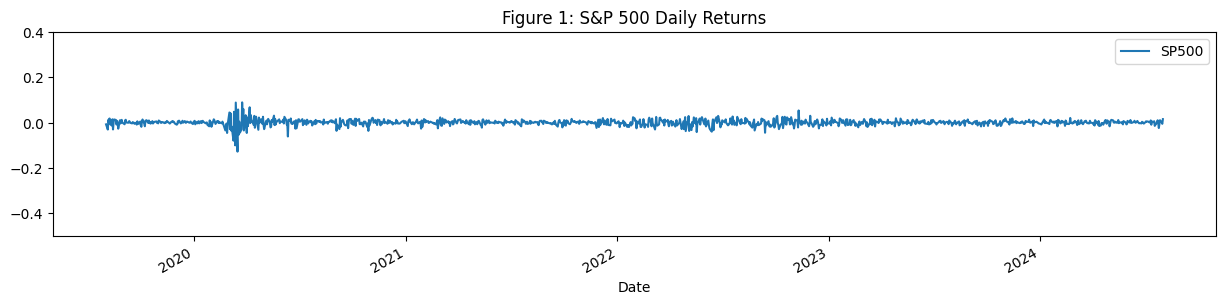
\includegraphics[width=\linewidth,height=0.6\textheight,keepaspectratio]{gfx/m2l2_notes_fig1_plot.png}
\par\smallskip{\small \textbf{Hình 1:} Lợi suất hàng ngày S\&P 500}
\end{figure}

\begin{figure}[H]
\centering
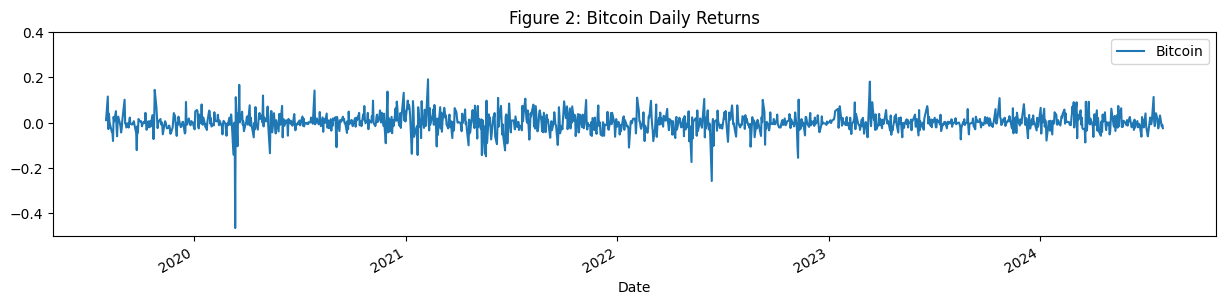
\includegraphics[width=\linewidth,height=0.6\textheight,keepaspectratio]{gfx/m2l2_notes_fig2_plot.png}
\par\smallskip{\small \textbf{Hình 2:} Lợi suất hàng ngày Bitcoin}
\end{figure}

Các biểu đồ trên cho thấy rõ ràng Bitcoin biến động (volatile) nhiều hơn bao nhiêu so với S\&P 500 và do đó tại sao phương sai/độ lệch chuẩn của lợi suất lại cao hơn nhiều.

Độ lệch chuẩn được ưu tiên hơn phương sai trong hầu hết các trường hợp vì phương sai là kết quả bình phương của các đơn vị lợi suất. Bằng cách lấy căn bậc hai của giá trị này và do đó thu được độ lệch chuẩn, kết quả sẽ ở cùng đơn vị với dữ liệu cơ sở, mà trong trường hợp này là lợi suất. Về mặt trực giác, điều này giúp nó dễ hiểu hơn nhiều.

Hãy ghi nhớ rằng độ lệch chuẩn thấp hơn không nhất thiết là được ưu tiên hơn khi xem xét các khoản đầu tư. Tất cả phụ thuộc vào sở thích rủi ro của nhà đầu tư. Rủi ro cao hơn có nghĩa là tiềm năng phần thưởng cao hơn. Hiểu được góc nhìn của nhà đầu tư là chìa khóa để xác định mức độ rủi ro nào mà một nhà đầu tư cảm thấy thoải mái.

\section{Hiệp phương sai và tương quan}

Chúng ta có thể so sánh hiệu suất của các cổ phiếu có các mức giá khác nhau bằng cách sử dụng lợi suất và độ lệch chuẩn. Làm thế nào chúng ta có thể xem xét hiệu suất chung của hai cổ phiếu? Đối với điều này, chúng ta chuyển sang hiệp phương sai (covariance) và tương quan (correlation). Chúng ta sẽ bắt đầu với hiệp phương sai:

\[\frac{\sum(x_{i}-\overline{x})(y_{i}-\overline{y})}{N-1}\]

trong đó

$x_i$ = giá trị của một quan sát của $x$ $y_i$ = giá trị của một quan sát của $y$ $\overline{x}$ = trung bình của $x$ $\overline{y}$ = trung bình của $y$ $N$ = số lượng quan sát

\textbf{Hiệp phương sai} cung cấp cho chúng ta một số hiểu biết về cách hai biến số di chuyển cùng nhau. Hiệp phương sai dương giữa lợi suất các cổ phiếu sẽ chỉ ra rằng khi một cổ phiếu tăng giá, cổ phiếu kia cũng vậy và ngược lại. Hiệp phương sai âm sẽ có nghĩa là hai cổ phiếu di chuyển nghịch chiều nhau, tức là khi cổ phiếu này tăng, cổ phiếu kia giảm.

Nhìn vào ma trận hiệp phương sai dưới đây cho ba tài sản của chúng ta, chúng ta có thể thấy rằng các tài sản này có mối quan hệ tích cực (dương) với nhau. Rất khó để hiểu được nhiều hơn thế với những con số này, do các đơn vị không được chuẩn hóa.

\subsection{Sử dụng ma trận hiệp phương sai}

Mặc dù hiệp phương sai hữu ích để xác định hướng của hai biến số cùng nhau, chúng ta có thể chuyển sang tương quan để có một phiên bản chuẩn hóa hơn của thước đo này. Hiện tại, khi thảo luận về tương quan, chúng ta sẽ sử dụng hệ số tương quan Pearson. Các loại tương quan khác sẽ được thảo luận trong một bài học tương lai.

\begin{lstlisting}[language=Python,escapeinside={(*@}{@*)}]
df.cov()
\end{lstlisting}

\begin{lstlisting}[escapeinside={(*@}{@*)}]
SP500
NASDAQ
Bitcoin




SP500
0.000181
0.000203
0.000200


NASDAQ
0.000203
0.000254
0.000253


Bitcoin
0.000200
0.000253
0.001726
\end{lstlisting}

Dưới đây là cách diễn giải nó:

\begin{itemize}
  \item Các giá trị trên đường chéo: Những giá trị này đại diện cho phương sai của mỗi tài sản. Ví dụ: 0.000181 là phương sai của lợi suất log hàng ngày của S\&P 500.
  \item Các giá trị ngoài đường chéo: Những giá trị này đại diện cho hiệp phương sai giữa hai tài sản khác nhau. Ví dụ: 0.000203 là hiệp phương sai giữa lợi suất log hàng ngày của S\&P 500 và NASDAQ.
\end{itemize}
Tất cả các giá trị đều dương, chỉ ra một mối quan hệ tích cực (cùng chiều) giữa lợi suất của các tài sản này. Điều này có nghĩa là khi lợi suất của một tài sản là số dương, lợi suất của các tài sản khác cũng có xu hướng dương.

\subsection{Sử dụng công thức hệ số tương quan Pearson}

Hệ số tương quan Pearson là một thước đo sức mạnh của mối quan hệ tuyến tính giữa hai biến số. Công thức như sau:

\[\rho_{_{X,Y}} = \frac{cov(X,Y)}{\sigma_{_{X}} \sigma_{_{Y}}}\]

trong đó

$cov$ = Hiệp phương sai $\sigma_{_{X}}$ = Độ lệch chuẩn của $X$ $\sigma_{_{Y}}$ = Độ lệch chuẩn của $Y$

Tương quan được sử dụng trong thống kê để định lượng mức độ mà hai biến số di chuyển trong một mối quan hệ tuyến tính với nhau. Tương quan có thể dao động từ -1 đến 1 (bao gồm cả hai đầu mút). Tương quan bằng 1 có nghĩa là tương quan hoàn hảo; các biến số di chuyển chính xác song hành cùng nhau. Sự song hành hoàn hảo đối với tương quan dương có nghĩa là nếu chúng ta biết biến X tăng, thì biến Y cũng tăng. Tương quan bằng -1 chỉ ra tương quan nghịch hoàn hảo. Đây cũng là sự song hành hoàn hảo, nhưng theo hướng ngược lại. Ở đây, nếu chúng ta biết biến X tăng, thì biến Y giảm. Tương quan bằng 0 chỉ ra rằng không có mối quan hệ tuyến tính nào có thể phân biệt được giữa hai biến số; do đó, sẽ không thể đưa ra dự đoán về một biến nếu biết biến kia. Trong trường hợp này, nếu chúng ta biết biến X tăng, thì biến Y có khả năng tăng hoặc giảm như nhau.

Một lợi ích của tương quan so với hiệp phương sai là tương quan được giới hạn từ -1 đến 1 trong khi hiệp phương sai có thể từ -vô cực đến +vô cực. Điều này làm cho hiệp phương sai trở thành một thống kê khó hiểu hơn về mặt trực giác. Tương quan cũng có tính tỷ lệ, điều này sẽ được hiển thị trong video bên dưới.

Hãy ghi nhớ rằng rất nhiều mô hình và khái niệm tài chính giả định một mức tương quan không đổi, nhưng điều này hiếm khi xảy ra. Tương quan thay đổi theo thời gian và thậm chí có khả năng thay đổi nếu bạn điều chỉnh khoảng thời gian mà từ đó bạn đang đo lường sự tương quan.

Khi so sánh các mức tương quan của các tài sản mà chúng ta đã và đang sử dụng cho đến nay, bạn có thể thấy nó vẽ ra một bức tranh rõ ràng hơn so với hiệp phương sai.

\begin{lstlisting}[language=Python,escapeinside={(*@}{@*)}]
round(df.corr(), 3)
\end{lstlisting}

\begin{lstlisting}[escapeinside={(*@}{@*)}]
SP500
NASDAQ
Bitcoin




SP500
1.000
0.947
0.358


NASDAQ
0.947
1.000
0.381


Bitcoin
0.358
0.381
1.000
\end{lstlisting}

Tất cả các biến số đều có mối quan hệ tích cực (dương), điều mà chúng ta đã thấy với ma trận hiệp phương sai trước đó. Ở đây, chúng ta cũng có thể thấy sức mạnh của các mối quan hệ: S\&P 500 có tương quan mạnh với NASDAQ vì chúng ta đã thu được hệ số tương quan Pearson là 0.947. Mối quan hệ giữa NASDAQ và Bitcoin vẫn là tích cực (dương) nhưng yếu hơn nhiều với hệ số tương quan Pearson là 0.381.

Khi chúng ta vẽ biểu đồ lợi suất giữa các biến số này, chúng ta có thể thấy bằng chứng về các mức tương quan ở trên, một cách trực quan:

\begin{lstlisting}[language=Python,escapeinside={(*@}{@*)}]
# (*@Tạo@*) (*@biểu@*) (*@đồ@*) (*@phân@*) (*@tán@*) (*@kèm@*) (*@đường@*) (*@hồi@*) quy
chart = sns.regplot(x="SP500", y="NASDAQ", data=df).set(
    (*@title="Hình@*) 3: (*@Lợi@*) (*@suất@*) (*@Hàng@*) (*@ngày@*) S&P 500 so (*@với@*) (*@Lợi@*) (*@suất@*) NASDAQ"
)

# (*@Thêm@*) (*@đường@*) (*@thẳng@*) (*@đứng@*) (*@tại@*) x=0 (*@và@*) (*@đường@*) (*@nằm@*) ngang (*@tại@*) y=0
plt.axvline(0, 0, 1, dash_capstyle="butt", linestyle="--", color="grey")
plt.plot([min(df.SP500), max(df.SP500)], [0, 0], linestyle="--", color="grey");
\end{lstlisting}

\begin{figure}[H]
\centering
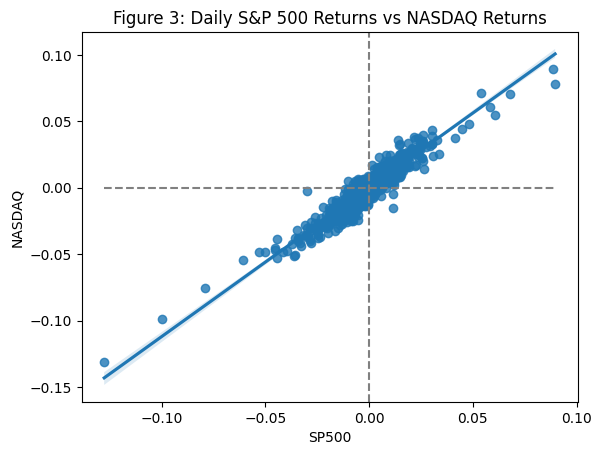
\includegraphics[width=\linewidth,height=0.6\textheight,keepaspectratio]{gfx/m2l2_notes_fig3_plot.png}
\par\smallskip{\small \textbf{Hình 3:} Lợi suất hàng ngày S\&P 500 so với lợi suất NASDAQ}
\end{figure}

Biểu đồ này hiển thị một cách trực quan mối quan hệ giữa lợi suất log hàng ngày của S\&P 500 và NASDAQ, bao gồm một đường hồi quy (regression line) đại diện cho mối quan hệ tuyến tính phù hợp nhất giữa hai biến số. Các đường đứt nét tại x=0 và y=0 giúp hình dung các mức lợi suất dương và âm cho mỗi tài sản. Mối quan hệ này cho thấy tương quan gần như hoàn hảo.

Bây giờ chúng ta hãy trực quan hóa mối quan hệ giữa lợi suất hàng ngày của S\&P 500 và Bitcoin.

\begin{lstlisting}[language=Python,escapeinside={(*@}{@*)}]
# (*@Tạo@*) (*@biểu@*) (*@đồ@*) (*@phân@*) (*@tán@*) (*@kèm@*) (*@đường@*) (*@hồi@*) quy
sns.regplot(x="SP500", y="Bitcoin", data=df).set(
    (*@title="Hình@*) 4: (*@Lợi@*) (*@suất@*) (*@Hàng@*) (*@ngày@*) S&P 500 so (*@với@*) (*@Lợi@*) (*@suất@*) Bitcoin"
)

# (*@Thêm@*) (*@đường@*) (*@thẳng@*) (*@đứng@*) (*@tại@*) x=0 (*@và@*) (*@đường@*) (*@nằm@*) ngang (*@tại@*) y=0
plt.axvline(0, 0, 1, dash_capstyle="butt", linestyle="--", color="grey")
plt.plot([min(df.SP500), max(df.SP500)], [0, 0], linestyle="--", color="grey");
\end{lstlisting}

\begin{figure}[H]
\centering
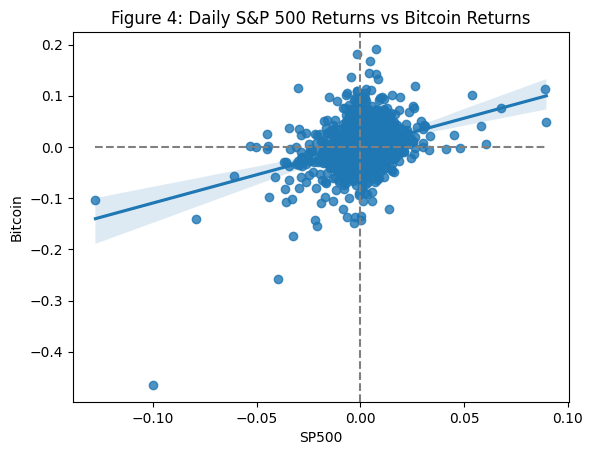
\includegraphics[width=\linewidth,height=0.6\textheight,keepaspectratio]{gfx/m2l2_notes_fig4_plot.png}
\par\smallskip{\small \textbf{Hình 4:} Lợi suất hàng ngày S\&P 500 so với lợi suất Bitcoin}
\end{figure}

Mối quan hệ ở đây phân tán hơn nhiều mặc dù mối quan hệ vẫn hơi tích cực (dương). Chúng được vẽ bằng phương thức \texttt{regplot()} của seaborn, phương thức này cũng hiển thị các khoảng tin cậy (confidence intervals) xung quanh đường hồi quy, như được thấy ở trên.

\subsection{Tỷ số Sharpe}

Có bất kỳ thống kê nào chúng ta có thể sử dụng để định lượng không chỉ lợi suất mà còn cả rủi ro không? Đối với điều này, chúng ta chuyển sang tỷ số Sharpe.

Tỷ số Sharpe (Sharpe ratio) cho phép nhà đầu tư hiểu được mối quan hệ giữa lợi suất của một khoản đầu tư và sự biến động của nó. Công thức như sau:

\[\text{Sharpe Ratio} = \frac{R_p - R_f}{\sigma_p}\]

trong đó

$R_p$ = Lợi suất của danh mục đầu tư $R_f$ = Lãi suất phi rủi ro $\sigma_p$ = Độ lệch chuẩn của danh mục đầu tư

Trong nhiều trường hợp khi lãi suất quá thấp, các nhà đầu tư sẽ giả định lãi suất phi rủi ro bằng 0, làm cho tỷ số trở thành:

\[\text{Sharpe Ratio} = \frac{R_p}{\sigma_p}\]

Bạn có nhận thấy điều gì về mẫu số không? Vâng, đúng vậy: chúng ta sử dụng độ lệch chuẩn ở đây để đại diện cho rủi ro.

Thước đo này được sử dụng như một cách chia tỷ lệ lợi suất của một khoản đầu tư tùy thuộc vào mức độ rủi ro được thực hiện. Nói cách khác, độ lệch chuẩn càng cao, lợi suất được điều chỉnh theo rủi ro (risk-weighted return) càng giảm. Hãy sử dụng cùng một ví dụ như trên với lợi suất hàng ngày của S\&P 500 và Bitcoin trong 5 năm qua.

\begin{lstlisting}[language=Python,escapeinside={(*@}{@*)}]
# (*@Tính@*) (*@tỷ@*) (*@số@*) Sharpe cho (*@cả@*) S&P 500 (*@và@*) Bitcoin
Sharpe_Ratio_SP500 = df["SP500"].mean() / df["SP500"].std()
Sharpe_Ratio_Bitcoin = df["Bitcoin"].mean() / df["Bitcoin"].std()

# In (*@kết@*) (*@quả@*)
print("Sharpe Ratio of S&P 500: ", round(Sharpe_Ratio_SP500, 5))
print("Sharpe Ratio of Bitcoin: ", round(Sharpe_Ratio_Bitcoin, 5))
\end{lstlisting}

\begin{lstlisting}[escapeinside={(*@}{@*)}]
Sharpe Ratio of S&P 500:  0.03699
Sharpe Ratio of Bitcoin:  0.03498
\end{lstlisting}

Dựa trên những kết quả này, S\&P 500 có Tỷ số Sharpe cao hơn một chút (0.03699) so với Bitcoin (0.03498). Điều này gợi ý rằng S\&P 500 đã mang lại mức lợi suất được điều chỉnh theo rủi ro tốt hơn một chút trong khoảng thời gian được phân tích.

Một sai sót lớn của tỷ số Sharpe là nó sử dụng độ lệch chuẩn của lợi suất ở mẫu số, điều này giả định rằng lợi suất có phân phối chuẩn. Điều này có thể không phải lúc nào cũng đúng - và thực tế hiếm khi xảy ra. Điều này sẽ được khám phá thêm trong một bài học tương lai.

\section{Bán phương sai}

Làm thế nào chúng ta có thể tinh chỉnh tỷ số Sharpe để đưa ra một thước đo thậm chí còn tốt hơn cho lợi suất điều chỉnh theo rủi ro? Bán phương sai (Semivariance) là câu trả lời. Bán phương sai, còn được gọi là rủi ro giảm giá (downside risk), là một phiên bản tinh tế hơn của độ lệch chuẩn. Độ lệch chuẩn xem xét cả rủi ro tăng giá (upside risk) và giảm giá của một khoản đầu tư. Hầu hết các nhà đầu tư, trừ khi bạn đang giao dịch bán khống (short), quan tâm nhiều hơn đến rủi ro giảm giá so với rủi ro tăng giá. Nói cách khác, nếu bạn đã mua một cổ phiếu và đang xem xét tỷ số Sharpe, bạn sẽ không muốn con số này bị phạt (penalize) vì cổ phiếu đó tăng giá mạnh đến mức nào. Hầu hết thời gian, một nhà đầu tư sẽ quan tâm nhiều hơn đến rủi ro giảm giá của một cổ phiếu.

\[\text{Semivariance} = \frac{1}{n} \sum_{r_i < \overline{r}}^{n} (r_i - \overline{r})^2\]

trong đó

$r_i$ = giá trị của một quan sát $\overline{r}$ = trung bình của tất cả các quan sát $n$ = số lượng quan sát

Có thể coi bán phương sai là một công cụ ước tính phương sai của các mức lợi suất thấp hơn mức trung bình của chúng. Điều này có thể được sử dụng để ước lượng mức lỗ trung bình mà một danh mục đầu tư có thể gánh chịu, giả định phân phối của lợi suất là phân phối chuẩn.

Ngược lại, nếu chúng ta bán khống (short) một chứng khoán, chúng ta vẫn có thể sử dụng bán phương sai, nhưng lần này, nó sẽ tập trung vào các mức lợi suất dương. Nếu chúng ta bán khống, sự sụt giảm về giá sẽ tạo ra phần tăng (upside), do đó chúng ta sẽ không muốn phạt sự biến động này trong tỷ số Sharpe của mình. Tuy nhiên, nếu có những độ lệch lớn theo hướng đi lên, thì điều này sẽ đóng góp vào bán phương sai. Tóm lại, bán phương sai sử dụng lợi suất dương hoặc lợi suất âm.

Bây giờ chúng ta hãy tính toán bán phương sai cho cả S\&P 500 và Bitcoin:

\begin{lstlisting}[language=Python,escapeinside={(*@}{@*)}]
# (*@Tính@*) (*@lợi@*) (*@suất@*) trung (*@bình@*) (*@của@*) (*@từng@*) (*@tài@*) (*@sản@*)
sp500mean = df["SP500"].mean()
BTCmean = df["Bitcoin"].mean()

# (*@Tính@*) (*@bán@*) (*@phương@*) sai (*@của@*) (*@từng@*) (*@tài@*) (*@sản@*)
sp500_semivariance = ((df[df["SP500"] < sp500mean]["SP500"] - sp500mean) ** 2).mean()
BTC_semivariance = ((df[df["Bitcoin"] < BTCmean]["Bitcoin"] - BTCmean) ** 2).mean()

# In (*@kết@*) (*@quả@*) (*@bán@*) (*@phương@*) sai
print("Semivariance of S&P 500: ", round(sp500_semivariance, 5))
print("Semivariance of Bitcoin: ", round(BTC_semivariance, 5))
\end{lstlisting}

\begin{lstlisting}[escapeinside={(*@}{@*)}]
Semivariance of S&P 500:  0.00021
Semivariance of Bitcoin:  0.00181
\end{lstlisting}

Đầu ra này cho thấy Bitcoin có bán phương sai cao hơn nhiều (0.00181) so với S\&P 500 (0.00021). Điều này chỉ ra rằng Bitcoin đã trải qua các sai lệch âm lớn hơn đáng kể so với mức lợi suất trung bình của nó, cho thấy rủi ro giảm giá cao hơn.

\section{Lợi suất cổ phiếu được phân phối như thế nào?}

Nhiều mô hình và lý thuyết xoay quanh cổ phiếu giả định một phân phối chuẩn (normal distribution). Chúng ta sẽ cố gắng xác định điều đó ở đây bằng một phân tích dựa trên dữ liệu. Các đặc tính của một phân phối Gaussian như sau:

\begin{itemize}
  \item Trung bình (mean), trung vị (median) và yếu vị (mode) đều như nhau.
  \item Dữ liệu đối xứng, có nghĩa là có số lượng quan sát bằng nhau ở cả hai phía của mức trung bình.
  \item Trong dữ liệu có phân phối chuẩn, 68.25\% tất cả các trường hợp rơi vào phạm vi +/- một độ lệch chuẩn từ mức trung bình, 95\% tất cả các trường hợp rơi vào phạm vi +/- hai độ lệch chuẩn từ mức trung bình và 99.7\% tất cả các trường hợp rơi vào phạm vi +/- ba độ lệch chuẩn từ mức trung bình.
\end{itemize}
Hãy bắt đầu bằng cách lấy 20 năm dữ liệu giá hàng ngày cho S\&P 500. Chúng ta sẽ sử dụng các phương pháp tương tự như chúng ta đã sử dụng trong một vài bài học trước để lấy dữ liệu này và sẽ tính toán lợi suất log ở đây.

Một cách nhanh chóng để làm điều này là xác định xem chúng ta có bao nhiêu điểm dữ liệu ở hai bên của mức trung bình ở đây. Chúng ta có hơn 5,000 điểm dữ liệu một chút. Đoạn code dưới đây lấy số lượng điểm dữ liệu lớn hơn mức trung bình và chia nó cho tổng số điểm dữ liệu. Điều này sẽ cho chúng ta tỷ lệ phần trăm các điểm dữ liệu lớn hơn mức trung bình.

\begin{lstlisting}[language=Python,escapeinside={(*@}{@*)}]
# (*@Ngày@*) (*@bắt@*) (*@đầu@*) (*@và@*) (*@ngày@*) (*@kết@*) (*@thúc@*)
start = datetime.date(2004, 8, 1)
end = datetime.date(2024, 8, 1)

# (*@Lấy@*) (*@dữ@*) (*@liệu@*)
# (*@Để@*) (*@chuyển@*) (*@đổi@*) (*@giữa@*) (*@tải@*) (*@dữ@*) (*@liệu@*) (*@trực@*) (*@tiếp@*) (*@và@*) (*@tải@*) (*@dữ@*) (*@liệu@*) (*@cục@*) (*@bộ,@*) 
# (*@bỏ@*) ghi (*@chú@*) (*@dòng@*) mong (*@muốn@*) (*@và@*) ghi (*@chú@*) (*@dòng@*) (*@còn@*) (*@lại.@*)
# (*@Lấy@*) (*@dữ@*) (*@liệu@*) Amazon, Ford (*@và@*) Bitcoin
#prices = pd.DataFrame(yfin.download(["^GSPC"], start, end, auto_adjust = False)["Adj Close"])
prices = pd.read_csv('FD_M2_L2_stocks_data.csv', index_col='Date', parse_dates=True)\
                    .loc[start:end].reindex(columns=["^GSPC"])

# (*@Loại@*) (*@bỏ@*) (*@giá@*) (*@trị@*) null (*@của@*) (*@các@*) (*@ngày@*) (*@cuối@*) (*@tuần@*) (*@và@*) (*@đổi@*) (*@tên@*) (*@cột@*) (*@để@*) (*@tên@*) (*@gọi@*) (*@trực@*) quan (*@hơn@*)
prices.dropna(inplace = True)
prices = prices.rename(columns={"^GSPC": "SP500"})
df = np.log(prices) - np.log(prices.shift(1))
df = df.iloc[1:, 0:]
\end{lstlisting}

\subsection{Lợi suất có đối xứng không?}

Một cách nhanh chóng để làm điều này là xác định xem chúng ta có bao nhiêu điểm dữ liệu ở hai bên của mức trung bình ở đây. Chúng ta có hơn 5,000 điểm dữ liệu ở đây một chút. Đoạn code dưới đây lấy số lượng điểm dữ liệu lớn hơn mức trung bình và chia nó cho tổng số điểm dữ liệu. Điều này sẽ cho chúng ta tỷ lệ phần trăm các điểm dữ liệu lớn hơn mức trung bình.

\begin{lstlisting}[language=Python,escapeinside={(*@}{@*)}]
(len(df[df.SP500 > df.SP500.mean()])) / (len(df))
\end{lstlisting}

\begin{lstlisting}[escapeinside={(*@}{@*)}]
0.5235446056030201
\end{lstlisting}

Đầu ra sẽ là một con số nằm giữa 0 và 1, đại diện cho tỷ lệ lợi suất hàng ngày của S\&P 500 lớn hơn lợi suất trung bình. Điều này có thể cho bạn một ý tưởng về độ xiên (skewness) của phân phối lợi suất. Giá trị gần 0.5 gợi ý một phân phối gần như đối xứng, trong khi giá trị lớn hơn đáng kể so với 0.5 gợi ý độ xiên âm (nhiều mức lợi suất nằm dưới mức trung bình hơn).

Chúng ta đang nhận được khoảng 52.6\% điểm dữ liệu lớn hơn mức trung bình, điều này cho thấy chúng ta có độ xiên hơi âm đối với tập dữ liệu này. Chúng ta không thể loại trừ lợi suất đối xứng dựa trên điều này vì nó chỉ là một mẫu dữ liệu và khá gần với mốc 50\%. Điều này gây khó khăn để nói chắc chắn liệu lợi suất của S\&P 500 có đối xứng hay không, nhưng ở đây vẫn có thể đưa ra một giả định hợp lý.

\subsection{Biến động có không đổi không?}

Đoạn code sau tính toán và vẽ biểu đồ độ lệch chuẩn trượt (rolling standard deviation) 50 ngày của lợi suất log S\&P 500, cung cấp một hình ảnh trực quan về sự biến động theo thời gian.

\begin{lstlisting}[language=Python,escapeinside={(*@}{@*)}]
# (*@Tính@*) (*@độ@*) (*@lệch@*) (*@chuẩn@*) (*@trượt@*)
vols = pd.DataFrame(df.SP500.rolling(50).std()).rename(columns={"SP500": "S&P 500 STD"})

# (*@đặt@*) (*@kích@*) (*@thước@*) (*@hình@*) (*@và@*) (*@vẽ@*) (*@các@*) (*@độ@*) (*@lệch@*) (*@chuẩn@*) (*@trượt@*)
plt.figure(figsize=(12, 5))
sns.lineplot(
    x="Date",
    y="S&P 500 STD",
    data=vols,
    label="S&P 500 50 day standard deviation rolling avg",
)
plt.show()
\end{lstlisting}

\begin{figure}[H]
\centering
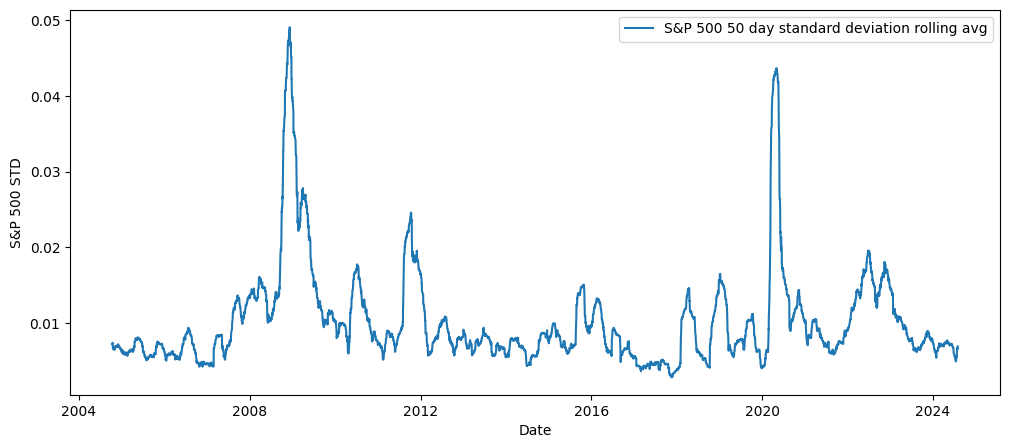
\includegraphics[width=\linewidth,height=0.6\textheight,keepaspectratio]{gfx/m2l2_notes_fig5_plot.png}
\par\smallskip{\small \textbf{Hình 5:} Độ lệch chuẩn trượt 50 ngày của lợi suất S\&P 500}
\end{figure}

Từ biểu đồ trên, có thể thấy rõ rằng biến động hoàn toàn không phải là không đổi. Điều này thêm một lớp phức tạp khác vào việc lập mô hình lợi suất cổ phiếu, đặc biệt là trong nhiều mô hình giả định mức biến động không đổi.

\section{Lợi suất cổ phiếu có phân phối chuẩn không?}

Phân phối chuẩn là một trong những phân phối phổ biến nhất được sử dụng trong việc lập mô hình các biến ngẫu nhiên. Quả thực, nhiều hiện tượng trong khoa học tự nhiên và xã hội có thể được lập mô hình bằng phân phối chuẩn. Một trong những lợi thế lớn của phân phối chuẩn là sự đơn giản của nó. Chúng ta có thể mô tả hoàn toàn một phân phối chuẩn thông qua hai con số: một cho tâm của phân phối và một cho độ bất định (uncertainty) xung quanh tâm đó. Con số đầu tiên đề cập đến mức trung bình, và con số thứ hai đề cập đến độ lệch chuẩn.

Khi chúng ta có hai con số này, chúng ta có thể đưa ra các suy luận, ước lượng các phân vị, tính toán xác suất để một điểm rơi vào một vùng, v.v. Nếu dữ liệu của chúng ta được biểu diễn tốt bằng phân phối chuẩn, thì chúng ta có thể tự tin sử dụng mức trung bình và độ lệch chuẩn để báo cáo mức lợi suất kỳ vọng và biến động của danh mục đầu tư. Nếu dữ liệu của chúng ta không được biểu diễn tốt bằng phân phối chuẩn, thì chúng ta cần tìm các phân phối khác phù hợp hơn. Do đó, ví dụ, khi chúng ta có một phân phối lợi suất cổ phiếu, chúng ta sẽ muốn bắt đầu đánh giá này bằng cách trực quan hóa lợi suất để xem chúng có vẻ chuẩn hay không. Tất nhiên, chúng ta có thể tiếp tục điều này bằng các đánh giá định lượng hơn thông qua việc chạy các kiểm định thống kê.

Chúng ta có thể trực quan hóa dữ liệu bằng phương thức \texttt{hist()}. Chúng ta truyền vào \texttt{bins = 100} dưới dạng tham số để xác định số lượng các nhóm (buckets) để đặt dữ liệu vào. Bạn càng có nhiều bins, dữ liệu sẽ trông càng chi tiết trong một biểu đồ tần suất (histogram). Việc tăng bins quá nhiều có thể dẫn đến dữ liệu hơi nhiễu, điều này sẽ khiến việc xác định phân phối chuẩn trở nên khó khăn hơn.

\begin{lstlisting}[language=Python,escapeinside={(*@}{@*)}]
df.hist(bins=100);
\end{lstlisting}

\begin{figure}[H]
\centering
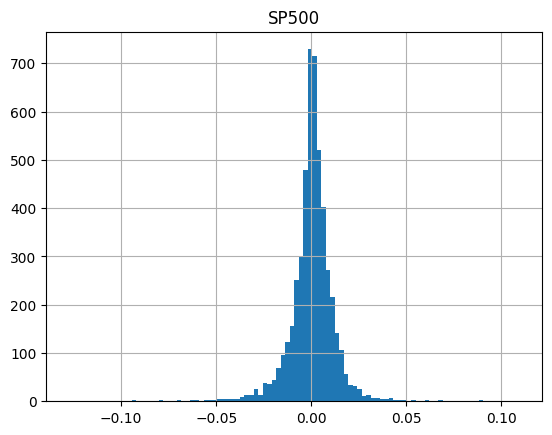
\includegraphics[width=\linewidth,height=0.6\textheight,keepaspectratio]{gfx/m2l2_notes_fig6_plot.png}
\par\smallskip{\small \textbf{Hình 6:} Biểu đồ tần suất (histogram) lợi suất của S\&P 500, NASDAQ và Bitcoin}
\end{figure}

Biểu đồ trên trông có vẻ như nó có thể có phân phối chuẩn, nhưng chúng ta cần khoa học hơn một chút để xác định xem điều đó có thực sự đúng hay không.

\subsection{Tiến hành kiểm định tính chuẩn}

Chúng ta có thể sử dụng phương thức \texttt{normaltest()} để xác định xem dữ liệu mẫu có thể phù hợp với một phân phối chuẩn hay không. Phương thức này sử dụng kiểm định tính chuẩn của D'Agostino và Pearson, kết hợp độ xiên (skew) và độ nhọn (kurtosis) để tạo ra một kiểm định tổng thể (omnibus test) về tính chuẩn.

\begin{lstlisting}[language=Python,escapeinside={(*@}{@*)}]
stats.normaltest((np.array(df.SP500)))
\end{lstlisting}

\begin{lstlisting}[escapeinside={(*@}{@*)}]
NormaltestResult(statistic=np.float64(1234.7310969195069), pvalue=np.float64(7.61288004534643e-269))
\end{lstlisting}

Đầu ra của đoạn code này bao gồm hai giá trị:

\begin{itemize}
  \item Thống kê (Statistic): Một thống kê kiểm định đo lường sự sai lệch so với tính chuẩn. Các giá trị cao hơn chỉ ra sự sai lệch lớn hơn.
  \item p-value: Xác suất quan sát được dữ liệu nếu nó thực sự có phân phối chuẩn. Một p-value nhỏ (thường nhỏ hơn 0.05) gợi ý rằng dữ liệu không có phân phối chuẩn.
\end{itemize}
Đầu ra ở trên cho thấy kết quả của kiểm định tính chuẩn D'Agostino và Pearson trên dữ liệu lợi suất log S\&P 500 của chúng ta. Thống kê 1234.73 là rất cao, chỉ ra một sự sai lệch đáng kể so với một phân phối chuẩn. P-value cực kỳ nhỏ (7.61e-269) cung cấp bằng chứng mạnh mẽ để bác bỏ giả thuyết không (null hypothesis) rằng dữ liệu có phân phối chuẩn. Nói một cách đơn giản hơn, kiểm định này gợi ý mạnh mẽ rằng lợi suất log hàng ngày của S\&P 500 trong tập dữ liệu của chúng ta không tuân theo một phân phối chuẩn.

\subsection{Kiểm định độ xiên và độ nhọn}

Như một bước kiểm định bổ sung, chúng ta có thể kiểm định độ xiên và độ nhọn của phân phối bằng kiểm định Jarque-Bera. Thống kê kiểm định sẽ luôn lớn hơn không. Thống kê kiểm định càng xa không, thì dữ liệu mẫu càng có nhiều khả năng không khớp với phân phối chuẩn.

May mắn cho chúng ta, Python có một thư viện khác để chúng ta sử dụng ở đây, điều này thực sự đơn giản hóa phân tích. Từ thư viện \texttt{scipy.stats}, chúng ta có thể áp dụng trực tiếp phương thức \texttt{jarque\_\allowbreak{}bera()} vào dữ liệu của mình để nhận được thống kê kiểm định.

\begin{lstlisting}[language=Python,escapeinside={(*@}{@*)}]
stats.jarque_bera((np.array(df.SP500))).pvalue
\end{lstlisting}

\begin{lstlisting}[escapeinside={(*@}{@*)}]
np.float64(0.0)
\end{lstlisting}

Một p-value nhỏ (thường nhỏ hơn 0.05) chỉ ra rằng dữ liệu có khả năng không được phân phối chuẩn. Đầu ra này chỉ ra rằng p-value từ kiểm định Jarque-Bera là 0.0 (hoặc cực kỳ gần bằng không). Điều này gợi ý mạnh mẽ rằng lợi suất log hàng ngày của S\&P 500 trong tập dữ liệu của bạn không có phân phối chuẩn.

\subsection{Phân phối Gaussian của chúng ta đổ vỡ ở đâu?}

Theo kiểm định tính chuẩn, dữ liệu của chúng ta không có phân phối chuẩn mặc dù biểu đồ tần suất trông có vẻ như vậy. Vậy tại sao dữ liệu lại trượt kiểm định tính chuẩn? Câu trả lời có thể là do đuôi béo (fat tails). Đuôi béo về cơ bản có nghĩa là các sự kiện cực đoan (cách mức trung bình +/- 3 độ lệch chuẩn) có nhiều khả năng xảy ra hơn so với những gì phân phối chuẩn ngụ ý.

Để xác định xem một con số cụ thể cách mức trung bình bao nhiêu độ lệch chuẩn, chúng ta cần sử dụng

\[\frac{X - \bar{X}}{\text{Sample standard deviation}}\]

Hãy thực hiện điều này cho mức tối thiểu (min) và tối đa (max) của dữ liệu mẫu:

\begin{lstlisting}[language=Python,escapeinside={(*@}{@*)}]
# (*@lợi@*) (*@suất@*) log (*@hàng@*) (*@ngày@*) (*@nhỏ@*) (*@nhất@*) (*@và@*) (*@lớn@*) (*@nhất@*)
dfMax = df.SP500.max()
dfMin = df.SP500.min()

# In (*@lợi@*) (*@suất@*) log (*@hàng@*) (*@ngày@*) (*@lớn@*) (*@nhất@*) (*@và@*) (*@nhỏ@*) (*@nhất@*)
print("Maximum return of sample data is: ", round(dfMax, 5))
print("Minimum return of sample data is: ", round(dfMin, 5))
print(' - - - - - - - - - -')

# (*@Tính@*) (*@số@*) (*@độ@*) (*@lệch@*) (*@chuẩn@*) so (*@với@*) (*@lợi@*) (*@suất@*) trung (*@bình@*)
num_dev_max = (df.SP500.max() - df.SP500.mean()) / df.SP500.std()
num_dev_min = (df.SP500.min() - df.SP500.mean()) / df.SP500.std()

# In num_dev_max (*@và@*) num_dev_min
print("Number of standard deviations from the mean for the maximum return: ", round(num_dev_max, 5))
print("Number of standard deviations from the mean for the minimum return: ", round(num_dev_min, 5))
\end{lstlisting}

\begin{lstlisting}[escapeinside={(*@}{@*)}]
Maximum return of sample data is:  0.10957
Minimum return of sample data is:  -0.12765
 - - - - - - - - - -
Number of standard deviations from the mean for the maximum return:  9.0497
Number of standard deviations from the mean for the minimum return:  -10.60025
\end{lstlisting}

Đầu ra này cung cấp những hiểu biết có giá trị về phân phối lợi suất log hàng ngày của S\&P 500, đặc biệt làm nổi bật sự hiện diện của các giá trị ngoại lệ (outliers) hoặc đuôi béo:

\begin{itemize}
  \item Lợi suất Tối đa và Tối thiểu: Mức lợi suất hàng ngày tối đa xấp xỉ 10.957\% và mức lợi suất hàng ngày tối thiểu xấp xỉ -12.765\% cho thấy phạm vi lợi suất được quan sát trong dữ liệu của chúng ta.
  \item Điểm Z (Z-scores): Điểm Z cho mức lợi suất tối đa và tối thiểu lần lượt là 9.05 và -10.6. Đây là những điểm Z cực kỳ cao, chỉ ra rằng cả mức lợi suất tối đa và tối thiểu đều là những giá trị ngoại lệ đáng kể, cách rất xa mức trung bình xét về độ lệch chuẩn.
\end{itemize}
Trong một phân phối chuẩn, bạn sẽ hiếm khi quan sát thấy các điểm dữ liệu cách mức trung bình hơn 3 độ lệch chuẩn. Những điểm Z cao này gợi ý rằng lợi suất hàng ngày của S\&P 500 có phần đuôi béo hơn so với một phân phối chuẩn, nghĩa là các sự kiện cực đoan (lợi suất dương hoặc âm lớn) có nhiều khả năng xảy ra hơn so với những gì được kỳ vọng theo tính chuẩn.

Thông tin này rất quan trọng đối với việc lập mô hình và quản trị rủi ro, vì việc dựa vào giả định về tính chuẩn có thể dẫn đến việc đánh giá thấp xác suất của các sự kiện cực đoan và các khoản lỗ tiềm ẩn.

Những độ lệch chuẩn này là khổng lồ khi so sánh với phân phối chuẩn. Chúng ta có thể thấy điều này một cách phân tích (analytically) khi chúng ta điền điểm z vào phương thức \texttt{norm.cdf()} để xác định xác suất giá trị này có thể xuất hiện trong một phân phối chuẩn:

\begin{lstlisting}[language=Python,escapeinside={(*@}{@*)}]
stats.norm.cdf(-10.60)
\end{lstlisting}

\begin{lstlisting}[escapeinside={(*@}{@*)}]
np.float64(1.4899011272964664e-26)
\end{lstlisting}

Điều này ngụ ý rằng cơ hội chúng ta có thể có một biến động thấp đến mức -12.77\% là 1.49e-26. Xác suất này thấp đến mức chúng ta sẽ không bao giờ kỳ vọng một sự kiện như thế này xảy ra trong đời mình. Chúng ta có nhiều sự kiện như thế này, như được minh họa bằng mức tối thiểu và tối đa.

Tiến xa hơn với ý tưởng này, dựa trên bảng phân phối chuẩn z, chúng ta sẽ kỳ vọng 99.7\% các điểm dữ liệu của chúng ta nằm trong phạm vi +/- 3 độ lệch chuẩn tính từ mức trung bình. Hãy xác định điều này cho dữ liệu mẫu của chúng ta. Trước tiên, chúng ta cần tìm các giá trị giới hạn ở mức +/- 3 độ lệch chuẩn:

\begin{lstlisting}[language=Python,escapeinside={(*@}{@*)}]
# (*@Tính@*) (*@các@*) (*@cận@*) (*@trên@*) (*@và@*) (*@cận@*) (*@dưới@*)
upper = (3 * df.SP500.std()) + df.SP500.mean()
lower = (-3 * df.SP500.std()) + df.SP500.mean()

# In (*@kết@*) (*@quả@*)
print("Upper bound: ", round(upper, 5))
print("Lower bound: ", round(lower, 5))
\end{lstlisting}

\begin{lstlisting}[escapeinside={(*@}{@*)}]
Upper bound:  0.03654
Lower bound:  -0.0359
\end{lstlisting}

Hai tính toán trên sẽ ngụ ý rằng 99.7\% tất cả các điểm dữ liệu của chúng ta nên nằm giữa -0.0359 và 0.03654.

Vì chúng ta có 5,031 điểm dữ liệu, chúng ta sẽ kỳ vọng khoảng 15 điểm (tức là .03\% của 5,031)  trong số đó nằm ngoài phạm vi đó nếu giả định về tính chuẩn được giữ vững. Bây giờ hãy xem thực tế chúng ta có bao nhiêu điểm. Hãy lọc DataFrame \texttt{df} để chọn các hàng mà lợi suất log hàng ngày của S\&P 500 nằm ngoài phạm vi của giới hạn trên (upper bound) và giới hạn dưới (lower bound). Sau đó, chúng ta sẽ đếm số lượng các điểm dữ liệu rơi vào phạm vi này:

\begin{lstlisting}[language=Python,escapeinside={(*@}{@*)}]
# (*@Tính@*) (*@số@*) (*@điểm@*) (*@dữ@*) (*@liệu@*)
len(df[(df["SP500"] < lower) | (df["SP500"] > upper)])
\end{lstlisting}

\begin{lstlisting}[escapeinside={(*@}{@*)}]
84
\end{lstlisting}

Đó là một số lượng giá trị ngoại lệ (outliers) đáng kể nếu xem xét rằng trong một phân phối chuẩn, bạn sẽ kỳ vọng chỉ khoảng 0.3\% các điểm dữ liệu rơi ra ngoài phạm vi được xác định bởi 3 độ lệch chuẩn từ mức trung bình.

Phát hiện này tiếp tục hỗ trợ kết luận từ các kiểm định tính chuẩn rằng lợi suất log hàng ngày của S\&P 500 không có phân phối chuẩn và có biểu hiện đuôi béo (fat tails). Sự hiện diện của các giá trị ngoại lệ này làm nổi bật tầm quan trọng của việc xem xét các phân phối thay thế và các thước đo rủi ro thay thế khi lập mô hình và phân tích dữ liệu tài chính.

\section{Các phân phối phi Gaussian (Non-Gaussian Distributions)}

Một phân phối thay thế tiềm năng mà chúng ta có thể sử dụng để dự báo lợi suất cổ phiếu là phân phối t của Student (Student's t-distribution). Phân phối này rất giống với phân phối chuẩn ngoại trừ việc nó có đuôi nặng hơn (heavier tails). Về mặt lý thuyết, điều này có vẻ hoàn hảo cho lợi suất hàng ngày dựa trên những gì chúng ta đã thấy cho đến thời điểm này.

Hãy tiến hành kiểm tra trực quan phân phối dữ liệu của chúng ta bằng cách xếp chồng phân phối chuẩn lên ước lượng mật độ hạt nhân (kernel density estimation - KDE) của lợi suất S\&P 500:

\begin{lstlisting}[language=Python,escapeinside={(*@}{@*)}]
# (*@Lấy@*) (*@mẫu@*) (*@từ@*) (*@phân@*) (*@phối@*) (*@chuẩn@*)
np.random.seed(222)
normal_dist = stats.norm.rvs(size=len(df["SP500"]), loc = df["SP500"].mean(), scale = df["SP500"].std())

# (*@Tạo@*) (*@thêm@*) (*@một@*) (*@cột@*) trong df (*@để@*) (*@dùng@*) (*@chức@*) (*@năng@*) (*@vẽ@*) KDE (*@của@*) pandas
df['Normal Sample'] = normal_dist

# (*@Vẽ@*) (*@các@*) (*@biểu@*) (*@đồ@*) KDE
df[['SP500', 'Normal Sample']].plot(kind = 'kde', xlim = (-0.1, 0.1), figsize = (12,4));
\end{lstlisting}

\begin{figure}[H]
\centering
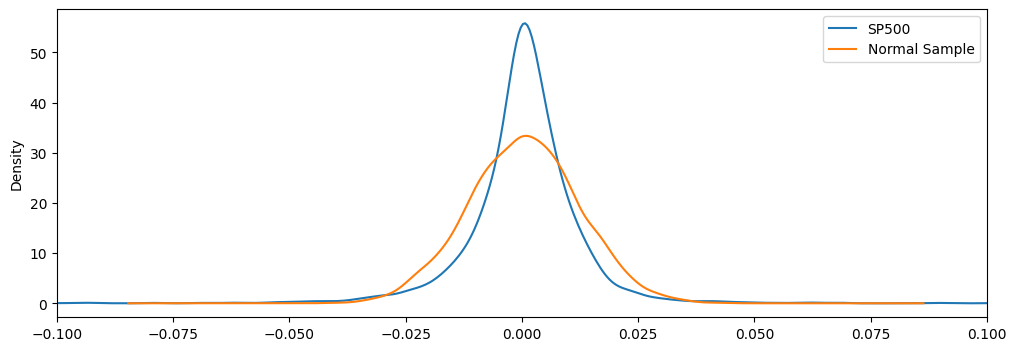
\includegraphics[width=\linewidth,height=0.6\textheight,keepaspectratio]{gfx/m2l2_notes_fig7_plot.png}
\par\smallskip{\small \textbf{Hình 7:} So sánh KDE của lợi suất S\&P 500 với mẫu rút từ phân phối chuẩn}
\end{figure}

Lợi suất của S\&P 500 có vẻ có đỉnh nhọn hơn nhiều (leptokurtic). Một phân phối leptokurtic (đỉnh nhọn) có đuôi béo hơn và đỉnh nhọn hơn so với phân phối chuẩn. Theo định nghĩa, các phân phối leptokurtic có độ nhọn (kurtosis) lớn hơn 3.

\begin{lstlisting}[language=Python,escapeinside={(*@}{@*)}]
df.SP500.kurt()
\end{lstlisting}

\begin{lstlisting}[escapeinside={(*@}{@*)}]
np.float64(13.18083916908493)
\end{lstlisting}

Thật vậy, độ nhọn của S\&P 500 lớn hơn đáng kể so với 3, xác nhận rằng phân phối lợi suất log hàng ngày của S\&P 500 là rất nhọn (highly leptokurtic).

Bây giờ, hãy kiểm tra xem phần đuôi của S\&P 500 có béo hơn phần đuôi của một phân phối chuẩn hay không. Đoạn code sau tạo ra một biểu đồ ước lượng mật độ hạt nhân (KDE) để so sánh các đuôi của lợi suất log hàng ngày thực tế của S\&P 500 với các đuôi của mẫu phân phối chuẩn được tạo ra. Nó tập trung vào đuôi bên trái (lợi suất âm) bằng cách thiết lập các giới hạn trục x thành (-0.075, -0.04).

\begin{lstlisting}[language=Python,escapeinside={(*@}{@*)}]
# Quan (*@sát@*) (*@phần@*) (*@đuôi@*)
df[['SP500', 'Normal Sample']].plot(kind = 'kde', xlim = (-0.075, -0.04), ylim = (-1, 2), figsize = (12,4));
\end{lstlisting}

\begin{figure}[H]
\centering
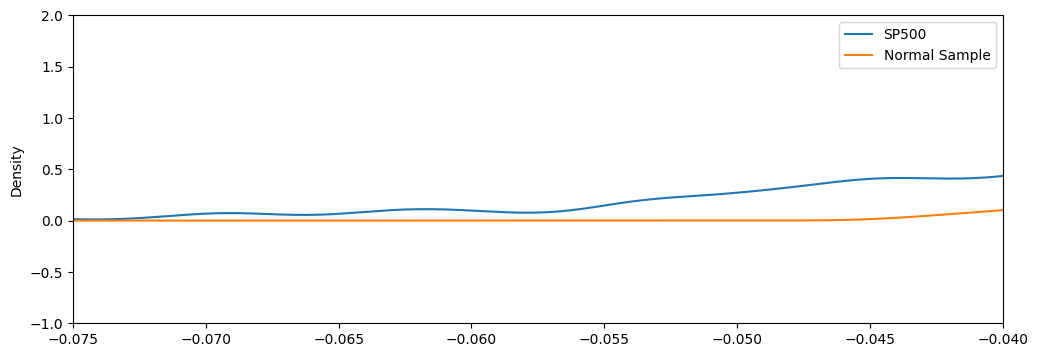
\includegraphics[width=\linewidth,height=0.6\textheight,keepaspectratio]{gfx/m2l2_notes_fig8_plot.png}
\par\smallskip{\small \textbf{Hình 8:} KDE lợi suất S\&P 500 và mẫu chuẩn, phóng to vào đuôi trái}
\end{figure}

Biểu đồ thu được cho thấy trực quan sự khác biệt ở phần đuôi của hai phân phối. Chúng ta quan sát thấy lợi suất thực tế của S\&P 500 có đuôi trái béo hơn phân phối chuẩn, cho thấy xác suất xảy ra các mức lợi suất âm lớn cao hơn. Hình ảnh này cung cấp thêm bằng chứng về tính không chuẩn của lợi suất S\&P 500 và sự hiện diện của các đuôi béo.

Ở giai đoạn này, chúng ta sẽ hiệu chỉnh các tham số của phân phối t của Student (Student's t-distribution) bằng phương pháp ước lượng hợp lý cực đại (Maximum Likelihood Estimation, MLE) để phân phối khớp sát với dữ liệu quan sát được. Đoạn code sau khớp một phân phối t của Student vào lợi suất log hàng ngày của S\&P 500 bằng \href{https://docs.scipy.org/doc/scipy/reference/generated/scipy.stats.fit.html}{ước lượng hợp lý cực đại (MLE)}, sau đó tạo biểu đồ KDE để so sánh phân phối t đã khớp với dữ liệu thực tế.

\begin{lstlisting}[language=Python,escapeinside={(*@}{@*)}]
# (*@Khớp@*) (*@phân@*) (*@phối@*) t (*@bằng@*) MLE
params = stats.t.fit(df.SP500)

# (*@Chúng@*) ta (*@vẽ@*) (*@phân@*) (*@phối@*) (*@đã@*) (*@khớp@*) (*@cùng@*) (*@với@*) KDE (*@của@*) (*@dữ@*) (*@liệu@*)
df['t-Sample *Fitted*'] = stats.t.rvs(*params, size = len(df))
df[['SP500', 't-Sample *Fitted*']].plot(kind = 'kde', figsize = (12,4), xlim = (-0.1, 0.1));
\end{lstlisting}

\begin{figure}[H]
\centering
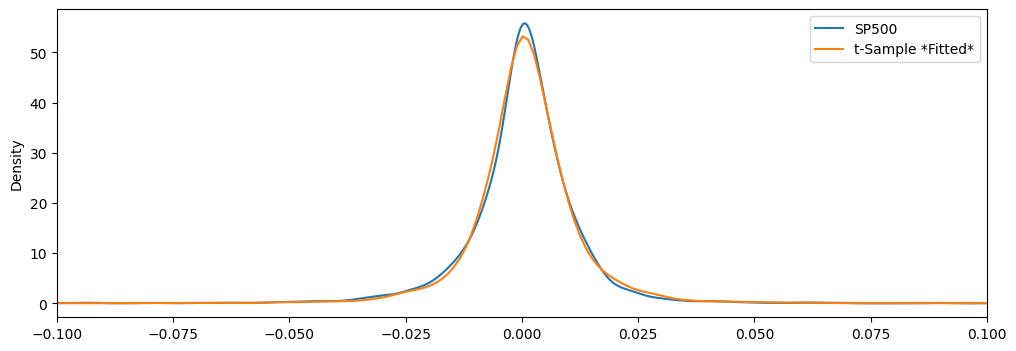
\includegraphics[width=\linewidth,height=0.6\textheight,keepaspectratio]{gfx/m2l2_notes_fig9_plot.png}
\par\smallskip{\small \textbf{Hình 9:} KDE lợi suất S\&P 500 và mẫu phân phối t đã khớp}
\end{figure}

Qua quan sát trực quan, có thể thấy rõ rằng dữ liệu tổng hợp được sinh ra từ phân phối t của Student đã khớp cho ra một mức xấp xỉ dữ liệu thực tế chính xác hơn so với những gì chúng ta có từ phân phối chuẩn.

Hãy kiểm tra lại phần đuôi một lần nữa. Chúng ta sẽ lại phóng to để quan sát mức độ gần nhau giữa đuôi trái của lợi suất log hàng ngày thực tế của S\&P 500 và đuôi trái của phân phối t của Student đã khớp:

\begin{lstlisting}[language=Python,escapeinside={(*@}{@*)}]
# (*@Vẽ@*) (*@vùng@*) (*@đuôi@*) (*@trái@*)
df[['SP500', 't-Sample *Fitted*']].plot(kind = 'kde', figsize = (12,4), xlim = (-0.075, -0.04), ylim = (-1, 2));
\end{lstlisting}

\begin{figure}[H]
\centering
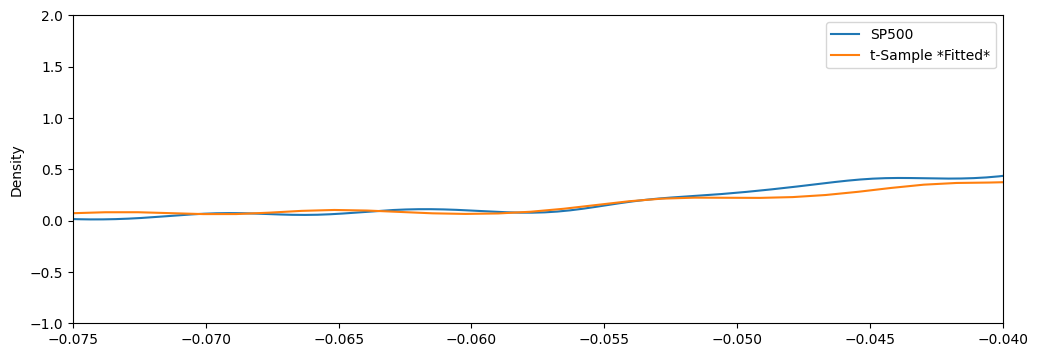
\includegraphics[width=\linewidth,height=0.6\textheight,keepaspectratio]{gfx/m2l2_notes_fig10_plot.png}
\par\smallskip{\small \textbf{Hình 10:} KDE lợi suất S\&P 500 và mẫu phân phối t đã khớp, phóng to vào đuôi trái}
\end{figure}

Lần này, phần đuôi dường như được phân phối t giải thích tốt hơn. Ở đây, chúng ta có thể quan sát thấy phân phối t đã khớp nắm bắt đuôi béo của lợi suất S\&P 500 chính xác hơn phân phối chuẩn. Điều này càng cho thấy sự phù hợp của phân phối t khi mô hình hóa dữ liệu tài chính có đuôi béo và khả năng xảy ra các sự kiện cực đoan.

\section{Kết luận}

Bài học này đã đề cập đến các chỉ số lợi suất và biến động ở mức bề mặt để so sánh các cổ phiếu. Chúng ta cũng đã thảo luận về các thước đo rủi ro giảm giá và những cách để so sánh đồng thời các tài sản tài chính khác nhau. Sau đó, chúng ta đi sâu vào các chỉ số nâng cao hơn được mô hình hóa bằng các phân phối thống kê khác nhau. Lần đầu tiên, chúng ta tập trung vào việc so sánh dữ liệu lợi suất cổ phiếu hàng ngày với các phân phối chuẩn. Chúng ta cũng đã đề cập đến những phân phối tiềm năng khác có thể dùng để mô hình hóa dữ liệu này.

\textbf{Tài liệu tham khảo}

\begin{itemize}
  \item D'Agostino, Ralph B. ``An Omnibus Test of Normality for Moderate and Large Size Samples.'' \emph{Biometrika} , vol. 58, no. 2, 1971, pp. 341--348, \url{https://doi.org/10.1093/biomet/58.2.341}.
\end{itemize}
Copyright 2024 WorldQuant University. This content is licensed solely for personal use. Redistribution or publication of this material is strictly prohibited.
